% !TEX encoding = UTF-8 Unicode
\documentclass[a4paper]{article}


\usepackage{color}
\usepackage{url}
\usepackage[T2A]{fontenc} % enable Cyrillic fonts
\usepackage[utf8]{inputenc} % make weird characters work
\usepackage{graphicx}
\usepackage{here} 



\usepackage[english,serbian]{babel}
%\usepackage[english,serbianc]{babel} %ukljuciti babel sa ovim opcijama, umesto gornjim, ukoliko se koristi cirilica

\usepackage[unicode]{hyperref}
\hypersetup{colorlinks,citecolor=green,filecolor=green,linkcolor=blue,urlcolor=blue}

\usepackage{listings}

%\newtheorem{primer}{Пример}[section] %ćirilični primer
\newtheorem{primer}{Primer}[section]

\definecolor{mygreen}{rgb}{0,0.6,0}
\definecolor{mygray}{rgb}{0.5,0.5,0.5}
\definecolor{mymauve}{rgb}{0.58,0,0.82}

\lstset{ 
  backgroundcolor=\color{white},   % choose the background color; you must add \usepackage{color} or \usepackage{xcolor}; should come as last argument
  basicstyle=\scriptsize\ttfamily,        % the size of the fonts that are used for the code
  breakatwhitespace=false,         % sets if automatic breaks should only happen at whitespace
  breaklines=true,                 % sets automatic line breaking
  captionpos=b,                    % sets the caption-position to bottom
  commentstyle=\color{mygreen},    % comment style
  deletekeywords={...},            % if you want to delete keywords from the given language
  escapeinside={\%*}{*)},          % if you want to add LaTeX within your code
  extendedchars=true,              % lets you use non-ASCII characters; for 8-bits encodings only, does not work with UTF-8
  firstnumber=1000,                % start line enumeration with line 1000
  frame=single,	                   % adds a frame around the code
  keepspaces=true,                 % keeps spaces in text, useful for keeping indentation of code (possibly needs columns=flexible)
  keywordstyle=\color{blue},       % keyword style
  language=Python,                 % the language of the code
  morekeywords={*,...},            % if you want to add more keywords to the set
  numbers=left,                    % where to put the line-numbers; possible values are (none, left, right)
  numbersep=5pt,                   % how far the line-numbers are from the code
  numberstyle=\tiny\color{mygray}, % the style that is used for the line-numbers
  rulecolor=\color{black},         % if not set, the frame-color may be changed on line-breaks within not-black text (e.g. comments (green here))
  showspaces=false,                % show spaces everywhere adding particular underscores; it overrides 'showstringspaces'
  showstringspaces=false,          % underline spaces within strings only
  showtabs=false,                  % show tabs within strings adding particular underscores
  stepnumber=2,                    % the step between two line-numbers. If it's 1, each line will be numbered
  stringstyle=\color{mymauve},     % string literal style
  tabsize=2,	                   % sets default tabsize to 2 spaces
  title=\lstname                   % show the filename of files included with \lstinputlisting; also try caption instead of title
}

\begin{document}

\title{Informacioni sistem za firmu Duma Group\\ \small{Seminarski rad u okviru kursa\\Informacioni sistemi\\ Matematički fakultet}}

\author{Miloš Miković, Anđela Križan, Milica Galjak, \\ Veronika Miljaković, Nikoleta Vukajlović}

%\date{9.~april 2015.}

\maketitle

\abstract{
%Ovde ide abstract
}

\tableofcontents

\newpage

\section{Uvod}

 Sistem je skup delova koji funkcionišu zajedno radi ostvarenja zajedničkog cilja ili svrhe. U domenu informatike i računarstva značajnu ulogu imaju \textbf{Informacioni sistemi}. Internacionalna federacija za obradu podataka (International Federation for Information Processing - IFIP) definiše informacioni sistem na sljedeći način: "Informacioni sistem je sistem koji prikuplja, pohranjuje, čuva, obrađuje i isporučuje informacije važne za organizaciju i društvo, tako da budu dostupne i upotrebljive za svakog ko se želi njima koristiti, uključujući poslovodstvo, klijente, zaposlene i ostale. Informacioni sistem aktivni je društveni sistem koji se može, ali i ne mora, koristiti      informacionom tehnologijom." 
    
 Predmet ovog rada je razvijanje informacionog sistema za firmu Duma Group iz Novog Sada. Izrađen je kao grupni projekat u okviru predmeta Informacioni sistemi, koji se sluša na prvoj godini master studija Matematičkog fakulteta u Beogradu.

\section{Analiza sistema}

Firma Duma Group se bavi organizovanjem proslava i događaja. U firminoj ponudi nalaze se brojne usluge čiji je cilj da obezbedi korisnicima sve ono što im je za njihove događaje potrebno. Među ovim uslugama su ketering, fotograf, prenosivi bar, slatki sto...

Prilikom formiranja ovog informacionog sistema poseban akcenat ćemo staviti na mađusobnu komunikaciju zaposlenih u firmi, kao i na komunikaciju sa klijentima, jer je to od velikog značaja za unapređenje firme.
    
Korisnici se registruju na sajt nakon čega stupaju u kontakt sa menadžerima firme. Menadžer treba od korisnika da dobije informacije o događaju koji korisnik pravi kako bi mu predložio adekvatnu uslugu. Nakon toga menadžer prenosi osoblju korisnikove želje. 
Ukoliko se korisnik opredeli za usluge keteringa ili prenosivog bara, osoblje ima zadatak da pripremi sadržaj koji je korisnik tražio i zadovolji sve njegove potrebe. Dostavljači nakon toga dostavljaju korisniku sav sadržaj.
Ukoliko se korisnik opredeli za usluge fotografa dogovaraju se svi potrebni detalji nakon čega fotografi pripremaju potrebnu opremu za događaj. Na dan događaja odlaze na mesto održavanja gde fotografišu i snimaju korisnika i njegove goste. Nakon toga sledi izrada fotografija. 
    
Osnovna svrha sistema je da omogući korisnicima da njihov događaj izgleda onako kako su zamislili i da mu za njega budu dostupne sve usluge koje su im potrebne. 
    
    \subsection{Učesnici u sistemu}
    
    \begin{enumerate}
        \item Klijent
        \item CEO menadžer
        \item Menadžer za ketering
        \item Menadžer za fotografiju
        \item Menadžer za prenosivi bar
        \item Osoblje
        \item Šef kuhinje
        \item Predstavnik foto studija
        \item Fotografi
        \item Barmen
        \item Gosti
        \item Dostavljač
    \end{enumerate}
    
    
\section{Slučajevi upotrebe}

% Ovo je moj deo - Miloš

\subsection{Registrovanje i prijavljivanje korisnika}

\begin{figure}[htp]
    \centering
    
\includegraphics[width=8cm]{Miloš/Miloš_Slučajevi_upotrebe_slike/Slucaj upotrebe _Registrovanje.jpg}
    \caption{Dijagram slučaja upotrebe Registracija korisnika}
    \label{fig:Registracija}
\end{figure}

\subsubsection{Registrovanje klijenta}

\begin{itemize}
    \item Kratak opis:
        \begin{itemize}
            \item Klijent se registruje kako bi mogao da koristi mogućnosti informacionog sistema Duma Group
        \end{itemize}
    \item Učesnici:
        \begin{itemize}
            \item Klijent koji želi da koristi usluge Duma Group sistema
        \end{itemize}
    \item Preduslov:
        \begin{itemize}
            \item Klijent poseduje računar ili pametni telefon i pristup Internetu
            \item Sistem je u funkciji
        \end{itemize}
    \item Postuslov:
        \begin{itemize}
            \item Klijent je registrovan i otvoren mu je nalog za korišćenje sistema
        \end{itemize}
    \item Glavni tok:
        \begin{enumerate}
            \item  Klijent otvara stranicu za registraciju odabirom određenog dugmeta na sajtu sistema
            \item Klijent čita uslove korišćenja sistema i prihvata ih
            \item Klijent popunjava formular unoseći tražene lične podatke. Kada zavši popunjavanje formulara pritiska dugme za registraciju
            \item Sistem obrađuje podatke i vrši validaciju
            \item Sistem kreira privremeni korisnički nalog
            \item Sistem šalje klijentu poruku na e-mail adresu unetu u formularu, postavlja predviđeno vreme za aktivaciju naloga i čeka
            \item Klijent proverava poštu i potvrđuje link za registraciju
            \item Sistem obeležava korisnički nalog kao aktivan i čuva podatke o nalogu
            \item Sistem obaveštava klijenta slanjem poruke na e-mail adresu klijenta da je nalog uspešno kreiran 
        \end{enumerate}
    \item Alternativni tok:
        \begin{itemize}
            \item Prilikom 2. koraka glavnog toka klijent odbija uslove korišćenja sistema. Sistem obaveštava korisnika da mora da prihvati date uslove korišćenja, vraća ga na 2. korak glavnog toka i onemogućava dalji tok registracije dok klijent ne prihvati date uslove.
            \item Prilikom 4. koraka glavnog toka ukoliko klijent nije uneo ispravne podatke, sistem obaveštava klijenta i proces se nastavlja od 3. koraka glavnog toka
            \item Ukoliko klijent nije prihvatio aktivacionu poruku u 7. koraku glavnog toka u određenom vremenskom periodu, sistem briše nalog i proces se završava.
            \item Ukoliko u 7. koraku glavnog toka klijent nije primio aktivacionu poruku on obaveštava sistem da mu ponovo pošalje poruku i proces se nastavlja od koraka 6. glavnog toka
        \end{itemize}
    \item Dodatne informacije:
        \begin{itemize}
            \item Potrebni podaci za registraciju su korisničko ime, lozinka, potvrda lozinke, broj kreditne kartice, ime, prezime, e-mail naloga, e-mail za povratak naloga ako se desi da je korisnik zaboravi lozinku ili korisničko ime, datum rodjenja korisnika, pol korisnika
            \item Ova registracija predstavlja registraciju klijenata sistema, postoji i registracija zaposlenih koja se vrši odvojeno
        \end{itemize}
\end{itemize}

\begin{figure}[htp]
    \centering
    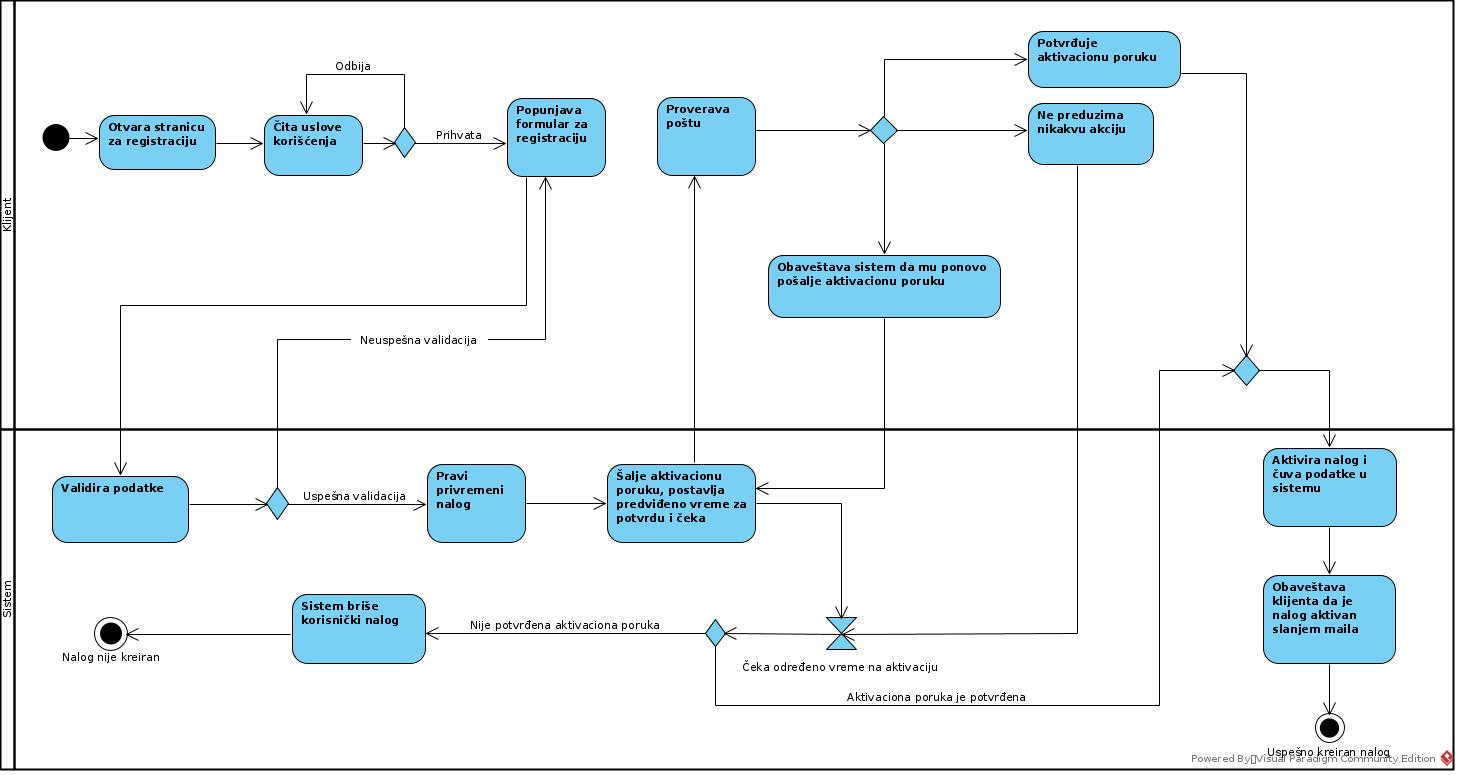
\includegraphics[width=10cm]{Miloš/Miloš_Dijagrami_aktivnosti_slike/Dijagram_aktivnosti_Registrovanje.jpg}
    \caption{Dijagram aktivnosti - Registrovanje korisnika}
    \label{fig:Registracija aktivnost}
\end{figure}


\subsubsection{Prijavljivanje korisnika}

\begin{figure}[htp]
    \centering
    
\includegraphics[width=8cm]{Miloš/Miloš_Slučajevi_upotrebe_slike/Slucaj upotrebe _Prijavljivanje.jpg}
    \caption{Dijagram slučaja upotrebe Prijavljivanje korisnika}
    \label{fig:Prijavljivanje}
\end{figure}

\begin{itemize}
    \item Kratak opis:
        \begin{itemize}
            \item Prethodno registrovani korisnik se prijavljuje na sistem
        \end{itemize}
    \item Učesnici:
        \begin{itemize}
            \item Registrovani korisnik koji želi da se prijavi na sistem
        \end{itemize}
    \item Preduslov:
        \begin{itemize}
            \item Korisnik mora biti registrovan u sistemu da bi se uspešno prijavio
            \item Korisnik poseduje računar ili pametni telefon i pristup Internetu
            \item Sistem je u funkciji
        \end{itemize}
    \item Postuslov:
        \begin{itemize}
            \item Korisnik je priavljen i može da koristi funkcionalnosti koje sistem pruža
        \end{itemize}
    \item Glavni tok:
        \begin{enumerate}
            %Možda da dodate početni korak da se otvara odgovarajuća stranica za
            %prijavu na sistem. Drugi korak može da se podeli na dva koraka. Sistem
            %proverava podatke i sistem prosleđuje korisnika dalje.
            \item Korisnik otvara stranicu za prijavljivanje
            \item Korisnik unosi svoje korisničko ime i šifru koju je koristio pri registraciji
            \item Sistem validira podatke
            \item Sistem sprovodi korisnika ka interfejsu aplikacije
        \end{enumerate}
    \item Alternativni tok:
        \begin{itemize}
            \item Ukoliko u 1. koraku glavnog toka korisnik ne može da se seti podataka za prijavljivanje obaveštava sistem da mu pošalje mail za oporavak. Sistem šalje mail korisniku, korisnik proverava mail i menja podatke u skladu sa instrukcijama koje je dobio u mailu. Sistem čuva izmene koje je korisnik napravio a proces se nastavlja od 1. koraka glavnog toka.
            \item Ukoliko u 3. koraku glavnog toka korisnički podaci nisu ispravni, sistem obaveštava korisnika o grešci i postavlja brojač neuspešnih pokušaja.
            Ako je brojač prethodno postavljen, njegova vrednost se uvećava za jedan. Proces se nastavlja od 2. koraka glavnog toka.
            \item Ukoliko sistem u 3. koraku glavnog toka određen broj puta ne uspe da validira korisničke podatke postavlja zabranu prijavljivanja za tog korisnika na određeni vremski period. Nakon isteka zabrane izvršavanje se nastavlja od 2. koraka glavnog toka.
        \end{itemize}
    \item Dodatne informacije:
        \begin{itemize}
            \item Zabrana prijavljivanja nakon nekoliko neuspešnih pokušaja postoji radi zaštite podataka i informacija sistema od eventualnih napada.
            \item Prijavljivanje se vrši na isti način i za klijente i za zaposlene u Duma Group preduzeću
        \end{itemize}
\end{itemize}


\begin{figure}[htp]
    \centering
    
\includegraphics[width=10cm]{Miloš/Miloš_Dijagrami_aktivnosti_slike/Dijagram_aktivnosti_Prijavljivanje.jpg}
    \caption{Dijagram aktivnosti - Prijavljivanje korisnika}
    \label{fig:Prijavljivanje aktivnost}
\end{figure}

%Ovo je moj deo - Veronika


\subsection{Prenosivi bar}

\begin{figure}[H]
    \centering
    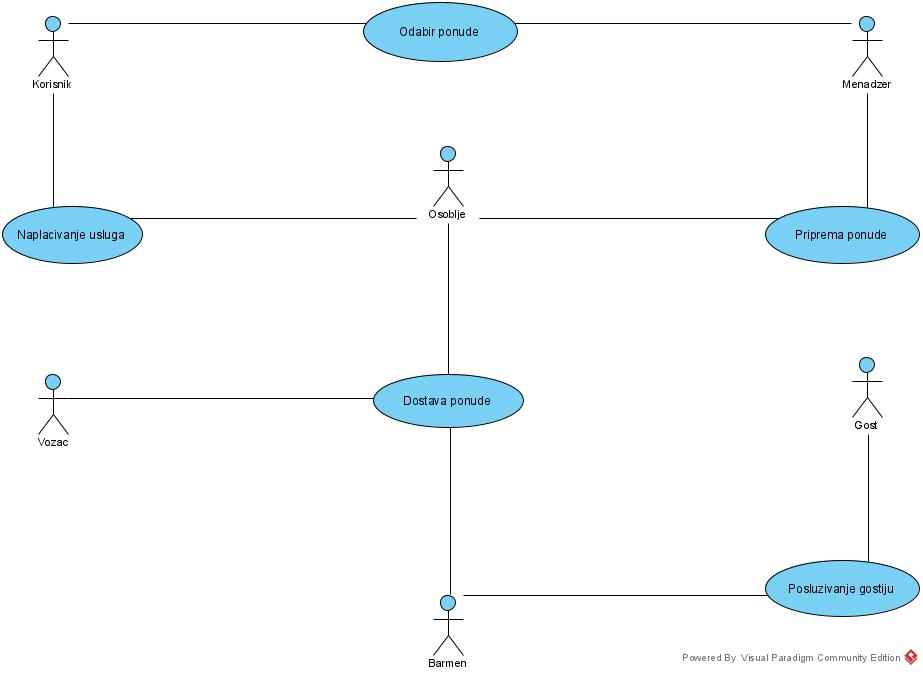
\includegraphics[width=8cm]{Slucaj upotrebe _ Prenosivi bar.jpg}
    \caption{Dijagram slučaja upotrebe Prenosivi bar}
    \label{fig:PrenosiviBar}
\end{figure}

\subsubsection{Odabir ponude}

\begin{itemize}
    \item Kratak opis:
        \begin{itemize}
            \item Klijent bira odgovarajuću ponudu u skladu sa događajem za koji mu je usluga potrebna
        \end{itemize}
    \item Učesnici:
        \begin{itemize}
            \item Klijent
            \item Menadžer za prenosivi bar
        \end{itemize}
    \item Preduslov:
        \begin{itemize}
            \item Klijent se registrovao na sajt
		    \item Na raspolaganju je spisak ponuda sa pratećim informacijama, slikama i snimcima
        \end{itemize}
    \item Postuslov:
        \begin{itemize}
            \item Klijent je odabrao odgovarajuću ponudu
            \item Menadžer je prihvatio odabir i zabeležio potrebne detalje u sistem
        \end{itemize}
    \item Glavni tok:
        \begin{enumerate}
		    \item Klijent se opredeljuje za uslugu ''Prenosivi bar''
		    \item Klijent preko sistema stupa u kontakt sa menadžerom za ovu uslugu
		    \item Klijent objašnjava menadžeru kog je tipa događaj i za šta mu je potreban bar
		    \item Menadžer mu preko sistema šalje ponudu iz ''Prenosivog bara'' sa pratećim informacijama o ceni, slikama i snimcima
		    \item Klijent bira sadržaj koji želi iz ponude i to se belezi u sistem
		    \item Klijent dogovara sa menadzerom detalje o datumu događaja, njegovom trajanju, dodatnim zahtevima i upitima
		    \item Menadžer beleži sve dogovorene detalje u sistemu i rezerviše odgovarajući datum
        \end{enumerate}
    \item Alternativni tok:
        \begin{itemize}
            \item Korak 5 - Sadržaj koji je klijent odabrao nije dostupan. U tom slucaju menadžer zamoli klijenta da odabere nešto drugo iz ponude i uputi ga na ponudu koja je slična onoj koju je tražio. Nakon toga klijent ponovo bira sadržaj za svoj događaj.
        \end{itemize}
\end{itemize}


\begin{figure}[H]
    \centering
    \includegraphics[width=8cm]{Dijagram aktivnost Prenosivi bar 1.jpg}
    \caption{Dijagram aktivnosti - Odabir ponude}
    \label{fig:PrenosiviBar}
\end{figure}


\subsubsection{Priprema ponude}

\begin{itemize}
    \item Kratak opis:
        \begin{itemize}
            \item Menadžer za Prenosivi bar prenosi ponudu osoblju koje nakon toga priprema ono što je zahtevano
        \end{itemize}
    \item Učesnici:
        \begin{itemize}
            \item Menadžer za prenosivi bar
            \item Osoblje
        \end{itemize}
    \item Preduslov:
        \begin{itemize}
            \item Klijent je odabrao svoju ponudu
		    \item Menadžer za prenosivi bar je prihvatio ponudu i zabeležio je u sistemu
        \end{itemize}
    \item Postuslov:
        \begin{itemize}
            \item Ponuda je pripremljena i spakovana za dostavu
        \end{itemize}
    \item Glavni tok:
        \begin{enumerate}
           \item Menadžer preko sistema šalje izabranu ponudu osoblju
		   \item Osoblje preuzima detalje o ponudi
	       \item Osoblje zaduženo za pripremu pića proverava u sistemu da li je svo piće koje je potrebno za događaj dostupno i ako jeste priprema odgovarajuću ponudu (donosi naručene flaše pića, čaše, slamčice, led i sve ostalo što je korisnik zahtevao)
	       \item Osoblje  zaduženo za nabavljanje prenosivog šanka, poslužaonika na kojima će se pića služiti i propratnih rekvizita za dekoraciju(cveće, table sa natpisima, baloni, ramovi za slikanje...) proverava u sistemu da li je sve potrebno za događaj dostupno i ako jeste priprema ono što je potrebno za tip događaja koji klijent pravi
	        \item Osoblje pakuje sav pripremljeni sadržaj u prevozno sredstvo tako da bezbedno stigne na dogovorenu lokaciju
        \end{enumerate}
    \item Alternativni tok:
        \begin{itemize}
            \item Koraci 3 i 4: Nešto od potrebnog sadržaja nije dostupno. U tom slučaju osoblje se obraća menadžeru kako bi nabavio ono što je klijent zahtevao
        \end{itemize}
\end{itemize}

\begin{figure}[H]
    \centering
    \includegraphics[width=8cm]{Dijagram aktivnosti_Prenosivi_bar}
    \caption{Dijagram aktivnosti - Priprema ponude}
    \label{fig:PrenosiviBar}
\end{figure}


\subsubsection{Dostava ponude}

\begin{itemize}
    \item Kratak opis:
        \begin{itemize}
            \item Ponuda je dovezena na potrebnu lokaciju i spremna za posluživanje
        \end{itemize}
    \item Učesnici:
        \begin{itemize}
            \item Dostavljač
            \item Osoblje
        \end{itemize}
    \item Preduslov:
        \begin{itemize}
            \item Sva potrebna roba je spakovana u prevozno sredstvo
		    \item Dostavljač je na raspolaganju	
        \end{itemize}
    \item Postuslov:
        \begin{itemize}
            \item Sve je postavljeno po dogovoru i događaj može da počne
        \end{itemize}
    \item Glavni tok:
        \begin{enumerate}
            \item Dostavljač dobije informaciju iz sistema gde treba odvesti porudžbinu i osoblje zaduženo za postavljanje
           \item Dostavljač odvozi robu i osoblje na dogovorenu adresu sat vremena pre početka događaja 
		    \item Osoblje montira prenosivi šank  
		    \item Osoblje ređa caše, flaše, poslužaonike na šank i dekoriše ga onako kako je u sistemu zabeleženo
		    
        \end{enumerate}
    
\end{itemize}

\begin{figure}[H]
    \centering
    \includegraphics[width=8cm]{Dijagram aktivnosti 3 Prenosivi bar.jpg}
    \caption{Dijagram aktivnosti - Dostava ponude}
    \label{fig:PrenosiviBar}
\end{figure}

\subsubsection{Posluživanje gostiju}

\begin{itemize}
    \item Kratak opis:
        \begin{itemize}
            \item Gosti dolaze do šanka gde im barmen sipa pića i pravi odgovarajuće koktele 
        \end{itemize}
    \item Učesnici:
        \begin{itemize}
            \item Menadžer za prenosivi bar
            \item Gosti
            \item Barmen
        \end{itemize}
    \item Preduslov:
        \begin{itemize}
            \item Menadžeru su dostupne informacije o događaju
            \item Barmenu su dostupne čaše, odgovarajuća 
		    pića i dodaci za određene koktele.
        \end{itemize}
    \item Postuslov:
        \begin{itemize}
            \item Svi gosti su usluženi na odgovarajući način
        \end{itemize}
    \item Glavni tok:
        \begin{enumerate}
            \item Menadžer preko sistema šalje barmenu informacije o adresi, trajanju i tipu događaja
            \item Barmen dobija navedene informacije
            \item Barmen dolazi na odgovarajuću adresu i priprema se za posao
            \item Barmen iz sistema čita spisak pića koje je klijent naručio i priprema ih
           \item Gost dolazi do šanka i preuzima piće koje je želeo od barmena
		   \item Barmen uslužuje sledećeg gosta
		  \end{enumerate}
		\textit{Koraci 5 i 6 se ponavljaju za svakog gosta koji priđe šanku sve do kraja događaja}
	
    \item Alternativni tok:
        \begin{itemize}
	      \item	Korak 5 : Piće koje gost traži je u međuvremenu popijeno. U tom slučaju barmen preporučuje gostu neka druga pića koja su dostupna i gost bira jedno od njih.

        \end{itemize}
\end{itemize}

\begin{figure}[H]
    \centering
    \includegraphics[width=8cm]{Dijagram aktivnost 4 Prenosivi bar}
    \caption{Dijagram aktivnosti - Posluživanje gostiju}
    \label{fig:PrenosiviBar}
\end{figure}

\subsection{Rad sa zaposlenima}

\begin{figure}[H]
    \centering
    \includegraphics[width=8cm]{Nina/Slucaj upotrebe rad sa zaposlenima.jpg}
    \caption{Dijagram slučaja upotrebe Rad sa zaposlenima}
    \label{fig:RegistracijaZ}
\end{figure}

\subsubsection{Registracija zaposlenog}

\begin{itemize}
    \item Kratak opis: 
    \begin{itemize}
        \item Administrator registruje zaposlenog koji nema otvoren nalog u sistem Douma Group. Sistem izvršava validaciju i vraća potvrdu o registraciji, ukoliko je uspešna.
    \end{itemize}
    \item Učesnici:
        \begin{itemize}
        \item Administrator
        \item Zaposleni
    \end{itemize}
    \item Preduslovi:
        \begin{itemize}
            \item Zaposleni nema kreiran nalog.
            \item Sistem je u funkciji.
        \end{itemize}
    \item Postuslovi:
        \begin{itemize}
            \item Zaposleni je registrovan u sistem i dobija informacije kako da ga koristi.
        \end{itemize}
    \item Glavni tok:
        \begin{enumerate}
            \item Zaposleni popunjava obrazac sa potrebnim podacima za registraciju.
            \item Zaposleni predaje obrazac administratoru.
            \item Administrator proverava da li su podaci validni.
            \item Administrator popunjava formular sa podacima koje je dobio.
            \item Administrator bira poziciju zaposlenog.
            \item Sistem šalje obaveštenje administratoru da potvrdi unos.
            \item Administrator potvrđuje podatke klikom na dugme.
            \item Sistem obaveštava administratora da je uspešno registrovan nalog.
            \item Administrator šalje zaposlenom uputstvo za korišćenje sistema.
        \end{enumerate}
    \item Alternativni tokovi:
        \begin{itemize}
            \item Korak 3 - Ukoliko je obrazac nepravilno popunjen (nedostaju neki podaci), administrator obaveštava zaposlenog gde je napravljena greška kako bi je ispravio. Proces se nastavlja u koraku 1.
        \end{itemize}
\end{itemize}

\begin{figure}[H]
    \centering
    \includegraphics[width=10cm]{Nina/DijagramAktivnostiRegistracijaZaposlenog.jpg}
    \caption{Dijagram aktivnosti registracije zaposlenog}
    \label{fig:RegistracijaZ}
\end{figure}


\subsubsection{Brisanje naloga zaposlenog}

\begin{itemize}
    \item Kratak opis: 
    \begin{itemize}
        \item Briše se nalog zaposlenog sa kojim je prekinut radni odnos.
    \end{itemize}
    \item Učesnici:
        \begin{itemize}
        \item CEO menadžer
        \item Administrator
    \end{itemize}
    \item Preduslovi:
        \begin{itemize}
            \item Sa zaposlenim je prekinut radni odnos.
            \item Sistem je u funkciji.
        \end{itemize}
    \item Postuslovi:
        \begin{itemize}
            \item Nalog je obrisan.
        \end{itemize}
    \item Glavni tok:
        \begin{enumerate}
            \item CEO menadžer šalje zahtev administratoru da obriše nalog.
            \item Administrator pokreće postupak brisanja naloga zaposlenog klikom na dugme za brisanje.
            \item Administrator popunjava informacije o tome da li je zaposleni svojevoljno dao otkaz ili ne.
            \item Administrator potvrđuje brisanje.
            \item Sistem potvrđuje nalog kao obrisan.
        \end{enumerate}
\end{itemize}

\begin{figure}[H]
    \centering
    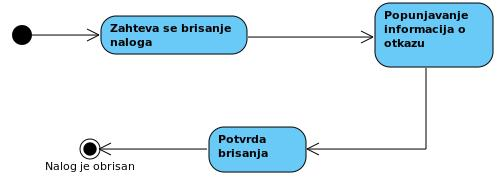
\includegraphics[width=8cm]{Nina/Dijagram_aktivnosti_brisanje_naloga.jpg}
    \caption{Dijagram aktivnosti brisanja naloga}
    \label{fig:RegistracijaZ}
\end{figure}

%%%%%%%%%%%%%%%%%%%%%%%%%%%%%%%%%%%%%%%%%%%%%%%%%%%%%%%%%%%%%%%%%%%%%%%%%%%%%%
% Ovo je moj deo - Andjela

\subsection{Fotografija}

\begin{figure}[htp]
    \centering
    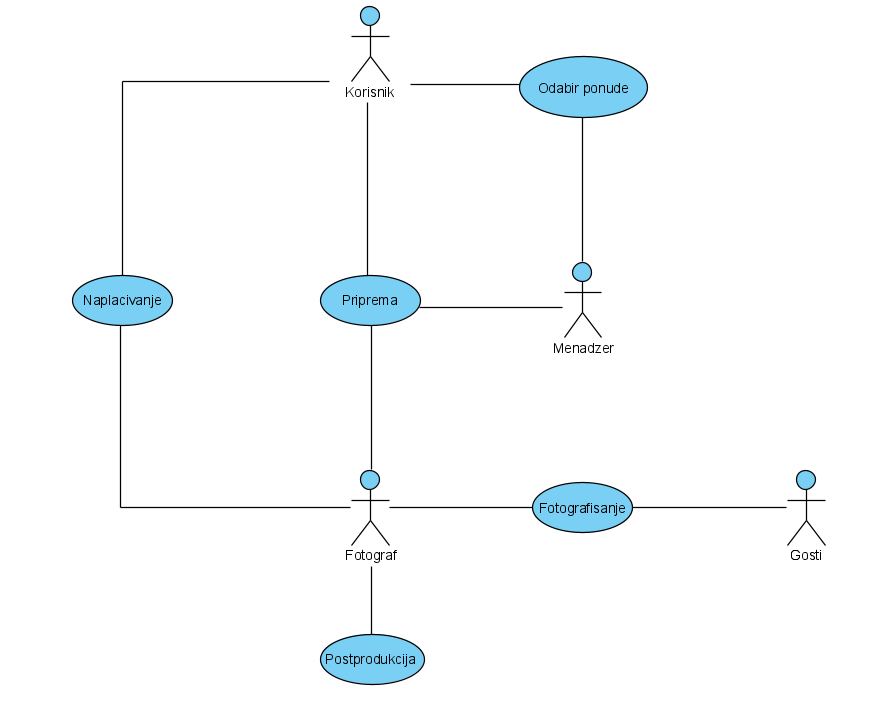
\includegraphics[width=8cm]{fotografija_dijagram1.png}
    \caption{Dijagram slučaja upotrebe Fotografija}
    \label{fig:PrenosiviBar}
\end{figure}

\subsubsection{Odabir ponude}
\begin{itemize}
    \item Kratak opis: 
    \begin{itemize}
        \item Korisnik bira ponudu fotografskih studija na osnovu njihovih foto izloga
    \end{itemize}
    \item Učesnici:
        \begin{itemize}
        \item Korisnik
        \item Predstavnik foto studija
        \item Menadžer za fotografiju
    \end{itemize}
    \item Preduslovi:
        \begin{itemize}
            \item Korisnik se registrovao na sajt
            \item Na raspolaganju je spisak ponuda različitih foto studija
        \end{itemize}
    \item Postuslovi:
        \begin{itemize}
            \item Korisnik je odabrao odgovarajuću ponudu
            \item Menadžer je obavešten o izboru foto studija
        \end{itemize}
    \item Glavni tok:
        \begin{enumerate}
            \item Korisnik se registruje na sajt
            \item Opredeljuje se za uslugu ''Fotografija''
            \item Bira ponudu nekog od predloženih foto studija
            \item Stupa u kontakt sa menadžerom za ovu uslugu
            \item Korisnik obaveštava menadžera kog je tipa događaj i za koji foto studio se odlučio na osnovu pregledanih ponuda 
            \item Korisnik i menadžer se dogovaraju oko detalja i dodatnih zahteva vezanih za događaj
        \end{enumerate}
    \item Alternativni tok:
        \begin{enumerate}
            \item Korisnik ima kontakt svog fotografa koji nije u saradnji sa firmom
            \item Stupa u kontakt sa menadžerom za ovu uslugu
            \item Obaveštava menadžera da ima svog fotografa, i daje menadžeru kontakt fotografa radi dalje organizacije
            \item Menadžer je prihvatio da sarađuje sa predloženim fotografom
        \end{enumerate}
\end{itemize}

\subsubsection{Priprema}
\begin{itemize}
    \item Kratak opis: 
    \begin{itemize}
        \item Menadžer obaveštava fotografa o rasporedu svečanosti
        \item Korisnik obaveštava o dodatnim zahtevima
    \end{itemize}
    \item Učesnici:
        \begin{itemize}
        \item Korisnik
        \item Predstavnik foto studija
        \item Menadžer za fotografiju
    \end{itemize}
    \item Preduslovi:
        \begin{itemize}
            \item Korisnik je izabrao foto studio i opredelio se za jednu ponudu
            \item Menadžer je prihvatio ponudu
        \end{itemize}
    \item Postuslovi:
        \begin{itemize}
            \item Tim fotografa iz foto studija su pripremili opremu u odnosu na zahtev
        \end{itemize}
    \item Glavni tok:
        \begin{enumerate}
            \item Korisnik obaveštava menadžera o svojim zahtevima 
            \item Menadžer obaveštava fotografe o rasporedu svečanosti
            \item Tim fotografa iz foto studija priprema opremu (rasvetu, kameru, dron...)
            \item Tim priprema plan fotografisanja u skladu sa zahtevima korisnika
            \item Na dan proslave, tim setuje opremu
        \end{enumerate}
\end{itemize}
\subsubsection{Fotografisanje}
\begin{itemize}
    \item Kratak opis: 
    \begin{itemize}
        \item Fotografi snimaju, sarađuju i menjaju pozicije kako bi zabeležili najvažnije trenutke
        \item Beleži se više materijala nego što je potrebno za finalni proizvod
    \end{itemize}
    \item Učesnici:
        \begin{itemize}
        \item Gosti
        \item Fotografi
    \end{itemize}
    \item Preduslovi:
        \begin{itemize}
            \item Oprema je setovana
            \item Fotografi su na pozicijama i čekaju da svečanost počne
        \end{itemize}
    \item Postuslov:
        \begin{itemize}
            \item Snimljen je sirovi materijal
            \end{itemize}
    \item Glavni tok:
        \begin{enumerate}
            \item Snimanje i fotografisanje slavlja sa gostima
            \item Fotografisanje slavljenika
        \end{enumerate}
    \item Alternativni tok:
        \begin{itemize}
            \item Ukoliko je u pitanju svadba (Post Wedding)
        \end{itemize}
        \begin{enumerate}
            \item Dan nakog proslave mladenci i fotografi idu na dogovorenu destinaciju radi fotografisanja
        \end{enumerate}
\end{itemize}
\subsubsection{Postprodukcija}
\begin{itemize}
    \item Kratak opis: 
    \begin{itemize}
        \item Pregled i obrada sirovog materijala 
    \end{itemize}
    \item Učesnici:
        \begin{itemize}
        \item Tim fotografa iz foto studija
    \end{itemize}
    \item Preduslov:
        \begin{itemize}
            \item Sakupljen je ceo master (sirovi materijal) spreman za obradu
        \end{itemize}
    \item Postuslov:
        \begin{itemize}
            \item Gotov je konačni proizvod
            \end{itemize}
    \item Glavni tok:
        \begin{enumerate}
            \item Pregled sirovog materijala
            \item Izrada finalnog proizvoda od sakupljenih fotografija. Finalni proizvod može biti fotoalbum, fotografije u elektronskoj formi, buk
            \item Izrada finalnog proizvoda od sakupljenih video snimaka. Izbor najuspešnijih kadrova. Finalni proizvod može biti spot(od 30s do 180s), film (kraća i duža verzija)
        \end{enumerate}
\end{itemize}
\subsubsection{Naplacivanje}
\begin{itemize}
    \item Kratak opis: 
    \begin{itemize}
        \item Po završetku postprodukcije, predstavnik foto studija se nalazi sa korisnikom radi primopredaje finalnog materijala i naplaćivanja usluge
    \end{itemize}
    \item Učesnici:
        \begin{itemize}
        \item Korisnik
        \item Fotograf
    \end{itemize}
    \item Preduslov:
        \begin{itemize}
            \item Finalni proizvod je gotov i spreman za isporuku
        \end{itemize}
    \item Postuslov:
        \begin{itemize}
            \item Usluga je plaćena
            \end{itemize}
    \item Glavni tok:
        \begin{enumerate}
            \item Fotograf predaje korisniku finalni proizvod
            \item Fotograf ispostavlja korisniku račun usluge
            \item Korisnik plaća uslugu
        \end{enumerate}
\end{itemize}
% kraj-Andjela
%%%%%%%%%%%%%%%%%%%%%%%%%%%%%%%%%%%%%%%%%%%%%%%%%%%%%%%%%%%%%%%%%%%%%%%%%%%%%%


%%%%%%%%%%%%%%%%
%pocetak-Milica

\subsection{Ketering}

\subsubsection{Prihvatanje porudzbine za dogadjaj}
\begin{itemize}
    \item Kratak opis:
    \begin{itemize}
        \item Menadzer obavestava osoblje kuhinje o samom dogadjaju. Osoblje odgovara o raspolozivosti za taj dogadjaj.
    \end{itemize}
\end{itemize}
  \begin{itemize}
        \item Ucesnici:
          \begin{itemize}
        \item Menadzer
    \end{itemize}
      \begin{itemize}
        \item Osoblje
    \end{itemize}
    \end{itemize}
      \begin{itemize}
        \item Preduslov:
          \begin{itemize}
        \item Menadzer je obavesten od strane klijenta o vrsti dogadjaja i detaljima porudzbine.
    \end{itemize}
    
    \end{itemize}
      \begin{itemize}
        \item Postuslov:
          \begin{itemize}
        \item Osoblje je informisano o predstvojecem dogadjaju.
    \end{itemize}
    \end{itemize}
      \begin{itemize}
        \item Glavni tok:
          \begin{enumerate}
              \item Menadzer salje mejl osoblju o datumu dogadjaja, tipu dogadjaja, detalje o samoj narudzbini keteringa.
        
              \item Svako od osoblja dobija mejl i proverava da li je zaposlen toga dana za neki drugi dogadjaj.
         
              \item Svako od osoblja odgovara menadzeru da li je slobodan toga dana.
        
              \item Menadzer ima spisak osoblja koje je slobodno za zakazani datum.
          
              \item Menadzer salje spisak osoblja sefu kuhinje.
          \end{enumerate}
    \end{itemize}
      \begin{itemize}
        \item Alternativni tok:
          \begin{itemize}
        \item Korak 4.-Ukoliko nema dovoljno osoblja za zakazani dogadjaj, menadzer stupa u kontakt sa klijentom, obavestava ga o tome i izlaze mu druge opcije kao sto su promena termina dogadjaja, manja kolicina porucene hrane...Ukoliko klijent prihvati druge opcije, menadzer ponovo salje mejl u kome su opisane promene u vezi dogadjaja.
    \end{itemize}
    \end{itemize}
\subsubsection{Priprema hrane za dogadjaj}
\begin{itemize}
    \item Kratak opis:
    \begin{itemize}
        \item Sef kuhinje zadaje zadatke za osoblje. Svako od osoblja procenjuje vreme koje mu je potrebno da zavrsi zadati deo posla i obavestava sefa kuhinje i tome. Priprema hrane.
    \end{itemize}
\end{itemize}
  \begin{itemize}
        \item Ucesnici:
          \begin{itemize}
        \item Sef kuhinje
    \end{itemize}
      \begin{itemize}
        \item Osoblje
    \end{itemize}
    \end{itemize}
      \begin{itemize}
        \item Preduslov:
          \begin{itemize}
        \item Sef kuhinje je obavesten o detaljima narudzbine.
   \end{itemize}
    
    \end{itemize}
      \begin{itemize}
        \item Postuslov:
          \begin{itemize}
        \item Narudzbina je gotova za dogovoreno vreme.
    \end{itemize}
    \end{itemize}
      \begin{itemize}
        \item Glavni tok:
          \begin{enumerate}
              \item Sef kuhinje ima spisak osoblja koji su raspolozivi za dogadjaj.
        
              \item U zavisnosti od vrste hrane koja je narucena i sposobnostima osoblja, podeljeni su zadaci osoblju od strane sefa kuhinje.
        
              \item Svako od osoblja procenjuje koliko vremena je potrebno da izvrsi zadati posao.
          
              \item Saopstava procenjeno vreme sefu kuhinje.
         
              \item U zavisnosti od procenjenog vremena osoblja i zakazanog termina dogadjaja, sef kuhinje zakazuje pocetak radnog vremena.
       
              \item U dogovoreno vreme, svako od osoblja pocinje sa izvrsavanjem svog dela posla.
          
              \item Ketering je spreman za dostavljanje.
          \end{enumerate}
    \end{itemize}
      \begin{itemize}
        \item Alternativni tok:
          \begin{itemize}
        \item Korak 5.- Ukoliko procenjeno vreme zavrsavanja posla prekoraci zakazano vreme dogadjaja, sef kuhinje preuzima deo posla koji ne bi bio gotov na vreme.
    \end{itemize}
    \end{itemize}
    
    
\subsubsection{Informacije o dostavi}
\begin{itemize}
    \item Kratak opis:
    \begin{itemize}
        \item Menadzer obavestava dostavljaca o terminu i lokaciji isporuke porucenog keteringa. Dostavljac potvrdjuje dostavu.
    \end{itemize}
\end{itemize}
  \begin{itemize}
        \item Ucesnici:
          \begin{itemize}
        \item Menadzer
    \end{itemize}
      \begin{itemize}
        \item Dostavljac
    \end{itemize}
    \end{itemize}
      \begin{itemize}
        \item Preduslov:
          \begin{itemize}
        \item Osoblje u kuhinji je zavrsilo posao na vreme.
        
   \end{itemize}
    
    \end{itemize}
      \begin{itemize}
        \item Postuslov:
          \begin{itemize}
        \item Dostavljac je obavesten o isporuci.
    \end{itemize}
    \end{itemize}
      \begin{itemize}
        \item Glavni tok:
          \begin{enumerate}
              \item Menadzer poziva dostavljaca i obavestava ga o detaljima isporuke.
          
              \item Dostavljac odgovara da li je slobodan da dostavi porudzbinu.
          \end{enumerate}
    \end{itemize}
      \begin{itemize}
        \item Alternativni tok:
          \begin{itemize}
        \item Korak 2.-Ukoliko dostavljac nije slobodan da dostavi narudzbinu, menadzer poziva nekog drugog dostavljaca.
    \end{itemize}
    \end{itemize}
    
\subsubsection{Dostava keteringa}
\begin{itemize}
    \item Kratak opis:
    \begin{itemize}
        \item Dostavljac prevozi u odredjeno vreme na odredjenu lokaciju poruceni ketering.
Klijent preuzima ketering.
    \end{itemize}
\end{itemize}
  \begin{itemize}
        \item Ucesnici:
          \begin{itemize}
        \item Klijent
    \end{itemize}
      \begin{itemize}
        \item Dostavljac
    \end{itemize}
    \end{itemize}
      \begin{itemize}
        \item Preduslov:
          \begin{itemize}
        \item Dostavljac je obavesten kada treba da dostavi porudzbinu i zna gde treba da dostavi porudzbinu.
   \end{itemize}
    
    \end{itemize}
      \begin{itemize}
        \item Postuslov:
          \begin{itemize}
        \item Porudzbina je dostavljena klijentu za dogadjaj.
    \end{itemize}
    \end{itemize}
      \begin{itemize}
        \item Glavni tok:
          \begin{enumerate}
              \item Dostavljac se informise kako moze da dodje na lokaciju dogadjaja.
        
              \item Procenjuje koliko mu je vremena potrebno da dostavi porudzbinu.
         
              \item U zavisnosti od procenjenog vremena odredjuje vreme polaska.
      
              \item Prevozi porucen ketering.
         
              \item Stize u dogovoreno vreme.
         
              \item Klijent preuzima isporuku.
          \end{enumerate}
    \end{itemize}
      \begin{itemize}
        \item Alternativni tok:
          \begin{itemize}
        \item Korak 2.-Dostavljac uzima u obzir nepredvidjene okolnosti na putu i obracunava vreme polaska shodno tome.
    \end{itemize}
    \end{itemize}
    
\begin{figure}[htp]
    \centering
    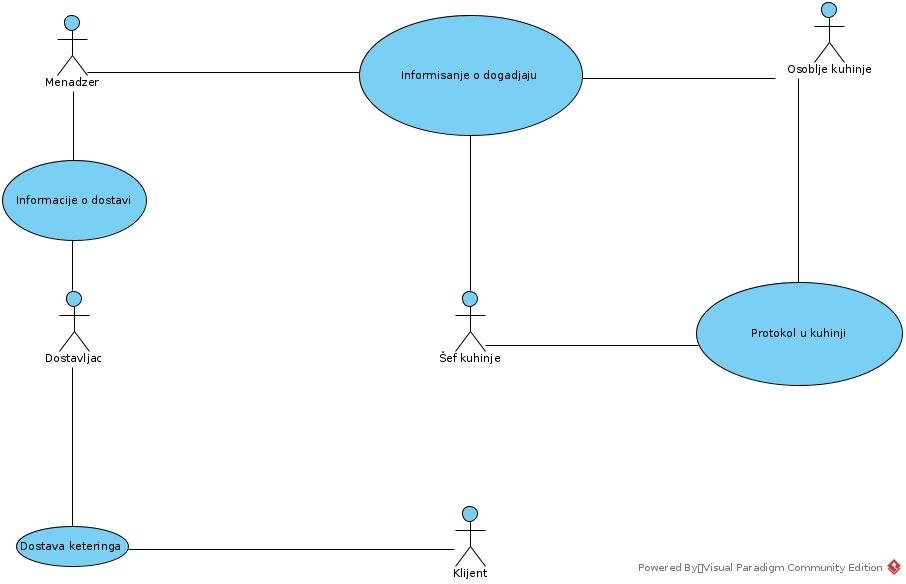
\includegraphics[width=8cm]{Ketering.jpg}
    \caption{Dijagram slučaja upotrebe Narucivanje keteringa}
    \label{fig:Ketering}
\end{figure}

%kraj-Milica
%%%%%%%%%%%%%%%%

\subsection{Naplata usluge}

\begin{figure}[H]
    \centering
    \includegraphics[width=8cm]{Nina/Naplata.jpg}
    \caption{Dijagram slučaja upotrebe Naplata usluge}
    \label{fig:RegistracijaZ}
\end{figure}

\begin{itemize}
    \item Kratak opis: 
    \begin{itemize}
        \item Po završetku usluge korisnik uplaćuje prethodno definisanu svotu novca.
    \end{itemize}
    \item Učesnici:
        \begin{itemize}
        \item Klijent
        \item Banka
        \item CEO menadžer
    \end{itemize}
    \item Preduslov:
        \begin{itemize}
            \item Usluga koju je klijent izabrao je završena.
            \item CEO menadžer ima uvid u broj računa firme.
            \item Klijent ima otvoren nalog za korišćenje aplikacije.
        \end{itemize}
    \item Postuslov:
        \begin{itemize}
            \item Transakcija je uspešno obavljena.
            \end{itemize}
    \item Glavni tok:
        \begin{enumerate}
            \item Klijent se prijavljuje na sajt firme Duma Group.
            \item Klijent uplaćuje definisanu svotu novca preko sajta. 
            \item Banka prosleđuje uplaćeni novac na račun firme.
            \item CEO menadžer dobija obaveštenje o uplati novca.
        \end{enumerate}
\end{itemize}

\begin{figure}[H]
    \centering
    \includegraphics[width=8cm]{Nina/Activity Diagram Naplata.jpg}
    \caption{Dijagram aktivnosti naplate usluge}
    \label{fig:RegistracijaZ}
\end{figure}

\end{document}
























